\documentclass{article}

\usepackage[utf8]{inputenc}
\usepackage[IL2]{fontenc}
\usepackage[slovak]{babel}
\usepackage{graphicx}
\usepackage{pdfpages}  % vloženie PDF
\usepackage{hyperref}

\title{Názov projektu}
\author{Yaroalav Nesteruk}
\date{07. október 2025}

\begin{document}
\maketitle

\section{Úvod}
Umelá inteligencia (AI) sa stala jednou z najdynamickejšie sa rozvíjajúcich oblastí informatiky.

\section{Ciele práce}
Cieľom práce je analyzovať aktuálne trendy a poukázať na praktické využitie.

\section{Použité metódy}
Analýza publikácií, porovnanie experimentov, syntéza poznatkov.

\section{Príloha PDF}
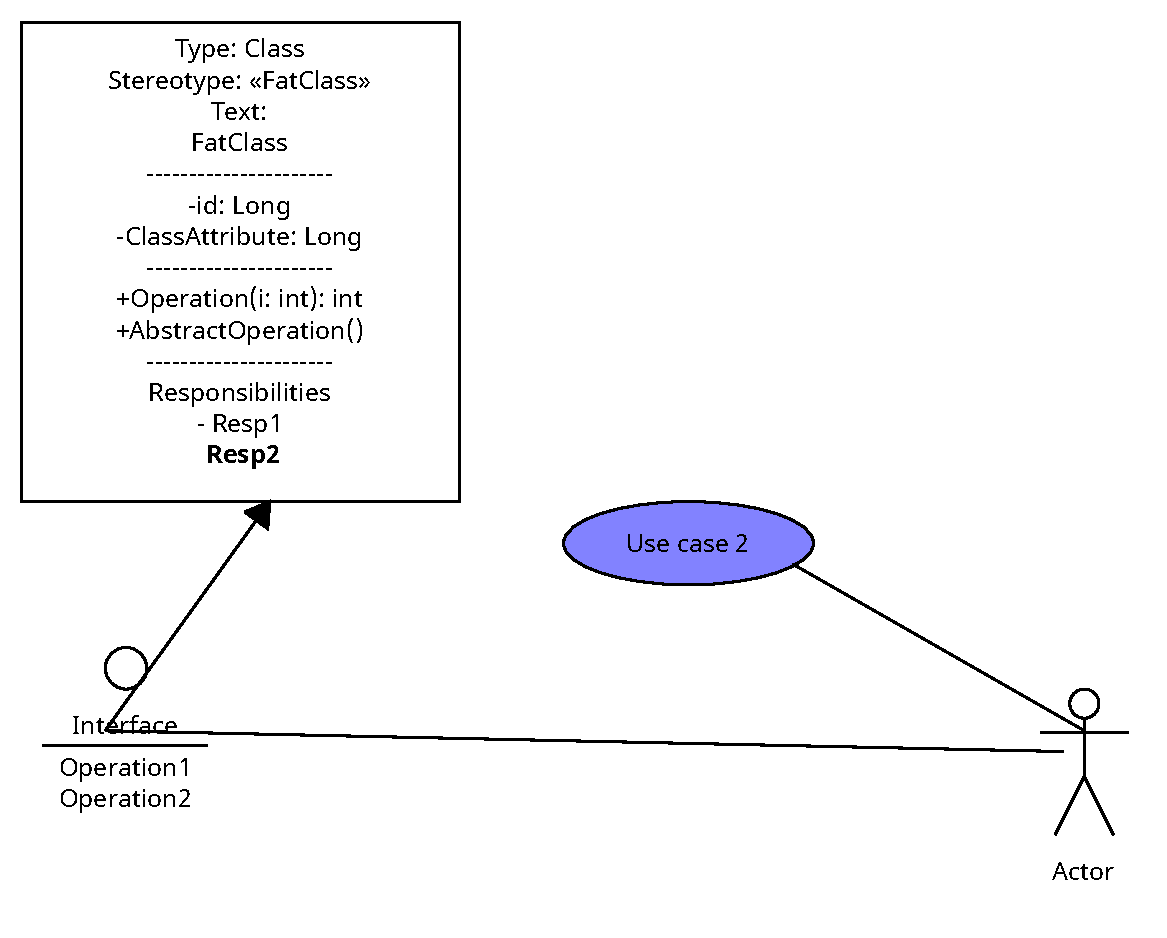
\includepdf[pages =-]{nieco.pdf}

\section{Záver}
AI bude hrať kľúčovú úlohu v rôznych sférach.

\section{Literatúra}
\begin{thebibliography}{9}
\bibitem{Goodfellow2016}
Ian Goodfellow, Yoshua Bengio, Aaron Courville. \emph{Deep Learning}. MIT Press, 2016.
\end{thebibliography}

\end{document}
